% 
% Introduction
%

Autism is an extremely complex developmental disorder diagnosed via the presence of a triad of symptoms including a qualitative impairment in social interactions, qualitative impairments in communication skills, and repetitive / stereotyped movements and behaviors~\nocite{RefWorks:98}(DSM-IV-TR, 2000).  The severity, and sometimes even presence, of the various symptoms in autism is highly variable between those afflicted with the disorder.  Due partly to this high variability, autism is generally seen as a spectrum of disorders known as autism spectrum disorders (ASD).  Alongside the requirements for an autism diagnosis are diverse and complex physical and behavioral profiles which continue to challenge every theories seeking to explain autistic behavior to date.  Steady progress is being made in early identification of behavioral characteristics of the disorder, as well as intervention techniques seeking to mitigate problematic behaviors.  However, no consensus has been reached concerning the neural basis of autism.  In the following we present a formal theoretical framework capable of explaining many aspects of autistic behavior in terms of specific neurological differences.  Specifically, a computational account is used to demonstrate how dysfunctional interactions between the midbrain dopamine system (DA) and the prefrontal cortex (PFC) could give rise to many of the behavioral patterns seen in ASD.

People with autism exhibit difficulties on a range of cognitive tasks.  These tasks assess such abilities as flexible adaptation, planning in order to reach a pre-specified goal, the generation of novel ideas, and determining the mental states of others~\cite{BennettoL:1996:AutismPlanningWCST,Ozonoff:1999:AutismStroopWCST,TurnerW:1999:AutismGenerativity,Baron-Cohen:1985:AutismTOM}.  Physically, abnormal gaits, problems initiating movements, abnormal sleep patterns, and an increased likelihood of developing a seizure disorder all accompany an autism diagnosis~\cite{RefWorks:99,RefWorks:100,RefWorks:101,RefWorks:102}.  Juxtaposed against the impairments of ASD exists a collection of spared, and sometimes enhanced, abilities in tasks such as the Embedded Figures Task~\cite{WitkinHA:1971:EFT} (EFT), where enhanced perceptual discrimination is regularly demonstrated people with autism~\cite{RefWorks:103,RefWorks:104}.  Along with the perceptual processing, superior and sometimes even savant abilities have been demonstrated in areas as diverse as mathematics, map memorization, music, artistic abilities, and date calculations~\cite{RefWorks:105,RefWorks:106,RefWorks:107,RefWorks:37}.   

The amazingly diverse profile demonstrated by people with ASD poses an incredibly daunting task for any single theory seeking to explain behavior in people with autism.  Indeed, the most widely acknowledged theories of ASD are generally circumscribed to account for very specific aspects of behavior.  For instance, an extremely pervasive theory in autism research has been the ``Theory of Mind'' (TOM) hypothesis, championed by Simon Baron-Cohen and Uta Frith~\cite{Baron-Cohen:1985:AutismTOM}, among others.  TOM posits that people with autism lack the ability to understand mental states, particularly intentional states (``I want'', ``I need'', ``I believe''), in others.  TOM is presented as a primary reason people with autism struggle socially. It is unclear, however, how the TOM hypothesis could be used to explain the patterns of deficits and spared abilities outside the social domain in people with ASD.  Instead, a separate theory is needed to account for this phenomenon. Often, the Weak Central Coherence (WCC) hypothesis is used to account for such abilities~\cite{RefWorks:37}.  In WCC, people with autism are viewed as enacting a unique processing style, rather than possessing a deficit, per se.  This style results in a ``piecemeal'' style of processing, rather than one that is more ``holistic''.  It is argued that a bias in favor of processing the pieces, or parts, of objects and situations can enhance performance when the task requires attention to the smaller details.  However, this bias comes at the price of a reduction in the ability to utilize more global, contextual, and gestalt information.  WCC posits that in ASD, there is a fundamental problem integrating the parts and pieces of a situation in order to understand the more global ``gist'' or context.  While WCC provides an account of some phenomena neglected by TOM, there are still other behavioral patterns that fall outside the explanatory range of both of these theories.  A third theory is needed to account for problems in planning, the flexible adaptation of behavior, and the generation of novel ideas.  All of these processes have been viewed as depending upon an executive processing system.  As such, dysfunction of these processes, known as Executive Dysfunction (ED), is believed by some to be a central feature of autism~\cite{HughesC:1994:AutismExecutiveDysfunction,HillEL:2004:AutismExecutiveDysfunction,Ozonoff:1991:AutismExecutiveDysfunction}.  

The combination of multiple theories, in this manner, have allowed theorists to cover the behavioral landscape of ASD.   It is not clear, however, that having a collection of relatively disjoint theories to explain different aspects of autism will foster the discovery of the underlying neural basis of this condition.  Furthermore, even if reliable underlying neural differences are identified and correlated with specific behavioral patterns exhibited by people with autism, we will still not understand how the specific neurological differences give rise to the behavior.  Knowing where the problem resides will not tell us why it results in autistic behavior.  

In the following we address this gap by employing the methods of computational cognitive neuroscience.  Computational models of cognition force the researcher to be explicit concerning the assumptions that are made, as well as the mechanisms employed, during scientific conjecture. The formal nature of these models allow us to form precise and testable hypotheses concerning the mechanisms responsible for the phenomena of interest. By incorporating explicit mechanistic characterizations of the underlying neurobiology, while capturing actual behavioral patterns, computational cognitive neuroscience models provide a means of bridging the conceptual valley between cognitive psychology and cognitive neuroscience in the domain of ASD research.

One general psychological question that has been explored using computational cognitive neuroscience techniques is how deliberate control over behavior (cognitive control) is instantiated within neural circuitry, as well as how this control is adjusted as environmental contingencies change (cognitive flexibility).  The PFC has been broadly implicated in both cognitive control and cognitive flexibility~\cite{Stuss:2000:WCSTLesion,Stuss:2001:StroopLesion}. Under some accounts, cognitive control is enacted via the active maintenance of abstract rule-like representations in PFC.  These sustained PFC representations provide a top-down task-appropriate processing bias to more posterior brain areas~\cite{CohenJD:1990:Stroop}. Biologically, the active maintenance of frontal control representations is supported by dense patterns of recurrent excitation in the PFC, as well as intrinsic maintenance currents~\cite{Goldman-RakicPS:1987:PFC_Maintenance}.  Computational analyses have shown that these two cognitive processes, cognitive control and cognitive flexibility, are at odds with one another.  Control requires robust and ongoing maintenance of a representation, where flexibility requires the ability to quickly and easily adapt these representations as task contingencies change.  This processing conflict suggests the need for a mechanism that intelligently toggles the PFC between a maintenance mode and an updating mode.  In order to avoid the introduction of an underspecified homunculus to control the PFC mode, computational accounts have sought a means for the PFC to learn when updating is appropriate.  This focus on learning has drawn attention to the dopamine system.   

Dopamine (DA), a neurotransmitter with diffuse projections throughout the brain, plays a vital role in contemporary models of prefrontal cortex function.  The dopamine system is seen as implementing a reinforcement learning algorithm, driving the learning of action sequences that lead to reward~\cite{MontaguePR:1996:Dopamine,BartoAG:1994:TDLearning}.  The mesolimbic dopamine system also modulates frontal pyramidal cells.  The DA projections to PFC are used to learn \emph{through experience} when cognitive control should be maintained and when it should be flexibly modified in order to succeed at the current task~\cite{BraverTS:2000:Control,RougierNP:2005:XT}. A useful analogy for this process is that of a “gate” in a fenced enclosure. When cognitive control must be strong, the gate is closed, keeping out distracting inputs that might compromise the needed PFC control signals. When the current control state is no longer appropriate, the gate opens, allowing the old control state to escape and permitting a new control representation to enter the PFC via its inputs.  Recent computational models of PFC function suggest that intelligent ``gating'' of control representations in PFC can be learned, through experience, via the specific error signal provided by DA neurons, as uncovered by electrophysiological studies~\cite{RougierNP:2005:XT,RougierNP:2002:TaskSwitching}. 

These computational accounts of PFC function, and interactions between PFC and the DA system, are potentially highly relevant for understanding the neural basis of behavioral patterns in ASD.  There is growing evidence for abnormal DA functioning in people with autism.  Aberrant levels of DA have been discovered in studies measuring DA via PET~\cite{FernellE:1997:AutismPET}, as well as more indirect measures such as HVA metaboloites~\cite{MartineauJ:1992:AutismDopamine}.  Clinical trials testing different drugs that modulate levels of DA in the brain have shown behavioral benefits as well~\cite{PoseyDJ:2000:AutismDopamine,TsaiLY:1999:AutismDopamine}. Further strengthening the importance of DA dysfunction in people with ASD are the numerous links between DA and behaviors tied to ASD symptomology.  These include increased prevalence of seizures, repetitive behaviors, and problems with skilled motor learning and control~\cite{RefWorks:1,RefWorks:3,RefWorks:5,RefWorks:2,RefWorks:109}.  In the following we use computational modeling methods to investigate and formalize what effect a DA deficit would have on the behavior of a developing individual, relating simulated behavioral results to actual data from studies of people with autism.  

%For example, within the executive profile of people with autism lies a paradox.  Executive functions are traditionally linked to processes believed to be largely instantiated within the frontal lobes, specifically the PFC.  In people with autism, the executive processes needed to instantiate control over behavior appears to be intact.  This is demonstrated by normal performance on tasks such as the classic Stroop test~\cite{StroopJR:1935:Interference,Ozonoff:1999:AutismStroopWCST}.  However, cognitive flexibility, the ability to appropriately adjust cognitive control as the environment changes, is impaired.  Poor performance on the perseverative error measure of the Wisconsin Card Sort Task (WCST) task is one common example of this impairment~\cite{BergEA:1948:WCST,Ozonoff:1999:AutismStroopWCST}.  If the PFC is central to both executive processes, cognitive flexibility and cognitive control, how can one be impaired while the other is spared and relatively robust?  One simple solution is to hypothesize separate mechanisms for each process.  This allows the PFC to function in a normal capacity, appropriately maintaining goal-like and attentional information in order to influence downstream processing.  The mechanism responsible for flexibly updating the contents of PFC is separate, consisting of neural signals arriving from the midbrain dopamine system.  In autism, it is this flexibility mechanism that we suggest is selectively damaged.  My modeling results suggest that weakening the influence of DA on the updating of PFC is sufficient to capture both qualitative and quantitative behavioral results on Stroop and WCST by people with autism.  This work is discussed in detail in Chapter~3.  

%This is just one example of how PFC / DA deficits can result in autistic-like behavior.  In the above case, ED is a direct result of perseveration on a ``rule'' (e.g. ``pay attention to the color'') that is actively maintained within the PFC.  In this case, the contents of PFC bias other cortical areas to produce behavior consistent with the actively maintained ``rule''.   There is no reason, however, the PFC needs to be restricted to only maintain rule-like items.  Indeed, the PFC is believed to be sufficiently general to encode any relevant aspect of an object or situation, and is not restricted to only verbally based ``rules''.  The active maintenance of these more general items allows the PFC to be cast as an important attentional mechanism, highlighting particular aspects and features of objects by providing a bias via up-modulation of cortical areas that are downstream from the PFC.  (Indeed, this is essentially the ``biased competition'' account of attention proposed by Desimone \& Duncan~\nocite{DesimoneR:1995:BiasedCompetition}(1995).)  Viewing the immediate cognitive result of perturbed DA / PFC interactions as perseverative \emph{attention} allows the scope of my theory to expand beyond ED in people with autism, encompassing a much broader range of phenomena.  These phenomena include many traditionally accounted for by attentional theories such as WCC theory and stimulus overselectivity. Stimulus overselectivity can be described as occuring when a overly restricted subset of the possible items in any situation gain control over behavior~\cite{RefWorks:110,RefWorks:111}.  The concept of attentional abnormalities in ASD has been noted by many researchers, including Leo Kanner in his seminal characterization of the disorder~\cite{KannerL:1943:Autism}, and therefore is not a novel idea.  Thus, the contribution of my work is not the novelty of noting attentional difficulties in people with autism.  Rather, it is the precise characterization of the mechanisms which give rise to the observed attentional difficulties.  Taking such a reductionistic approach allows us to provide a general framework explaining multiple aspects of behavior as well as physical manifestations of the disorder in people with ASD.  

%Another major aim of my research is to investigate the effect of overly perseverative attention, resulting from perturbed DA / PFC interactions, on learning and generalization.  Behavioral therapy and intervention techniques trying to mitigate autistic symptoms are extremely concerned with the generalization and transfer of skills learned during therapeutic sessions to novel settings.   In people with autism, stimulus overselectivity opposes the ability to generalize by restricting the attended features to an overly restricted subset of all the possible available items in any given situation.  If the restricted subset of features is not present in new situations where the same behavior is expected, generalization will be poor.  In other words, people with autism tend to associate overly specific, often idiosyncratic, aspects of a situation with the desired behavior.  This leads to problems using the learned behavior in novel contexts that do \emph{not} contain the associated and restricted subset of the learning context~\cite{RefWorks:89}.  Stimulus overselectivity has been operationalized using an operant conditioning paradigm~\cite{RefWorks:110}. (See Figure~\ref{OS-Task}.)  A compound stimulus, consisting of an auditory, visual, and tactile component, is associated with a reward if a lever is pressed.  After the initial stimulus / response association training, each individual component of the stimulus is presented separately. The control group demonstrated equal responding to each of the individual components.  The group of children with autism, however, tended to respond to only one of the three possible cues, demonstrating overselective responding.  In Chapter~4 we provide modeling results that demonstrate how flexible and proper updating of the contents of PFC is important for learning the associations between all stimulus components and reward.  This model demonstrates how overly perseverative modulation from a PFC-like mechanism results in more overselective responding, as compared with when the PFC is able to flexibly switch between dimensions.  A recent study demonstrating that overselectivity can be induced in normally developing individuals simply by inducing a working memory load during the task~\cite{RefWorks:112} provides further support.      

In this chapter we investigate the degree to which a single deficit, a dysfunctional dopaminergic system, can account for many of the patterns of behavior demonstrated by people with autism.  This investigation makes use of the methods of computational cognitive neuroscience, producing formal models that demonstrate how dopamine dysfunction can produce the behavioral patterns of interest.  By focusing on a single neurological mechanism with diverse behavioral effects, this approach provides a level of inter-theoretic reduction not found in many current theories seeking to explain autism.  The implications of the research expand beyond fundamental theorizing, potentially providing an improved understanding of the successes and failures of interventions utilized to reduce overselectivity and foster the generalization of learned behaviors in people with ASD.

%\begin{figure}
%\begin{center}
%	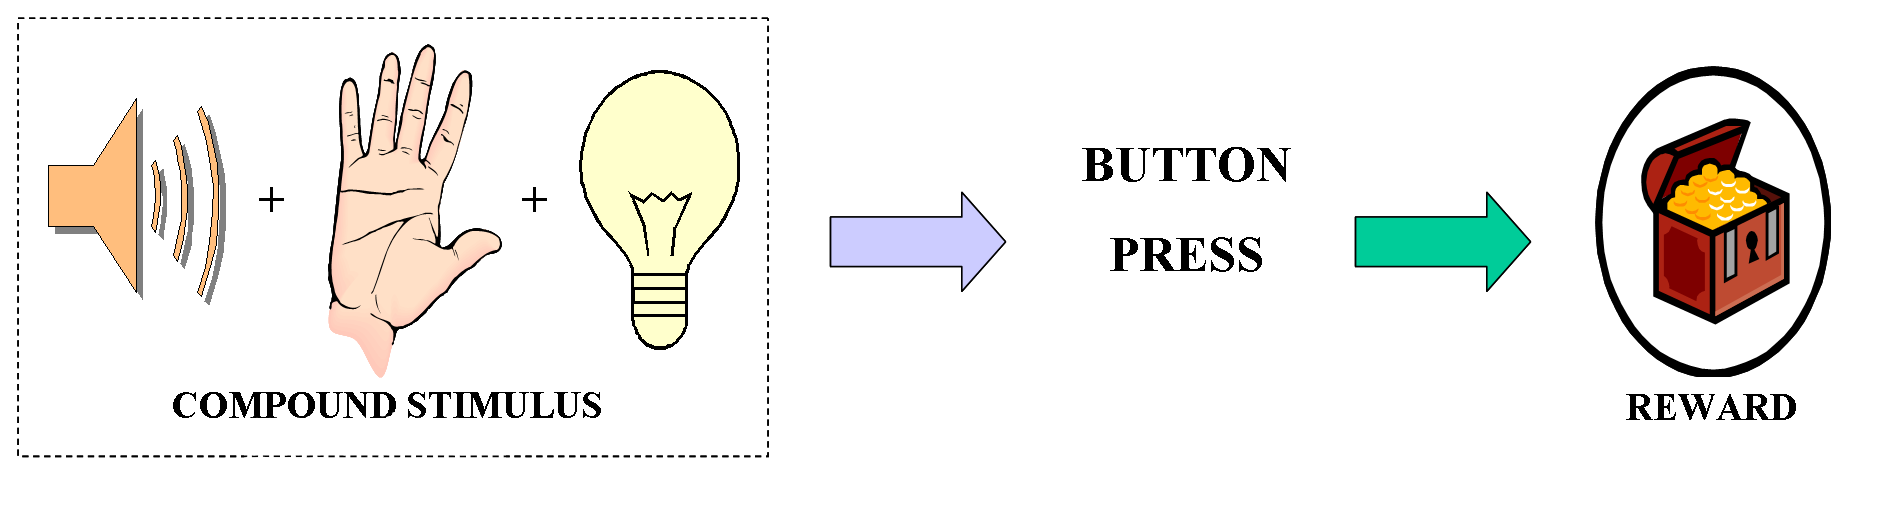
\includegraphics[width=85mm]{figures/compound_stimulus.eps}
%-----------------------------------------------------------
%	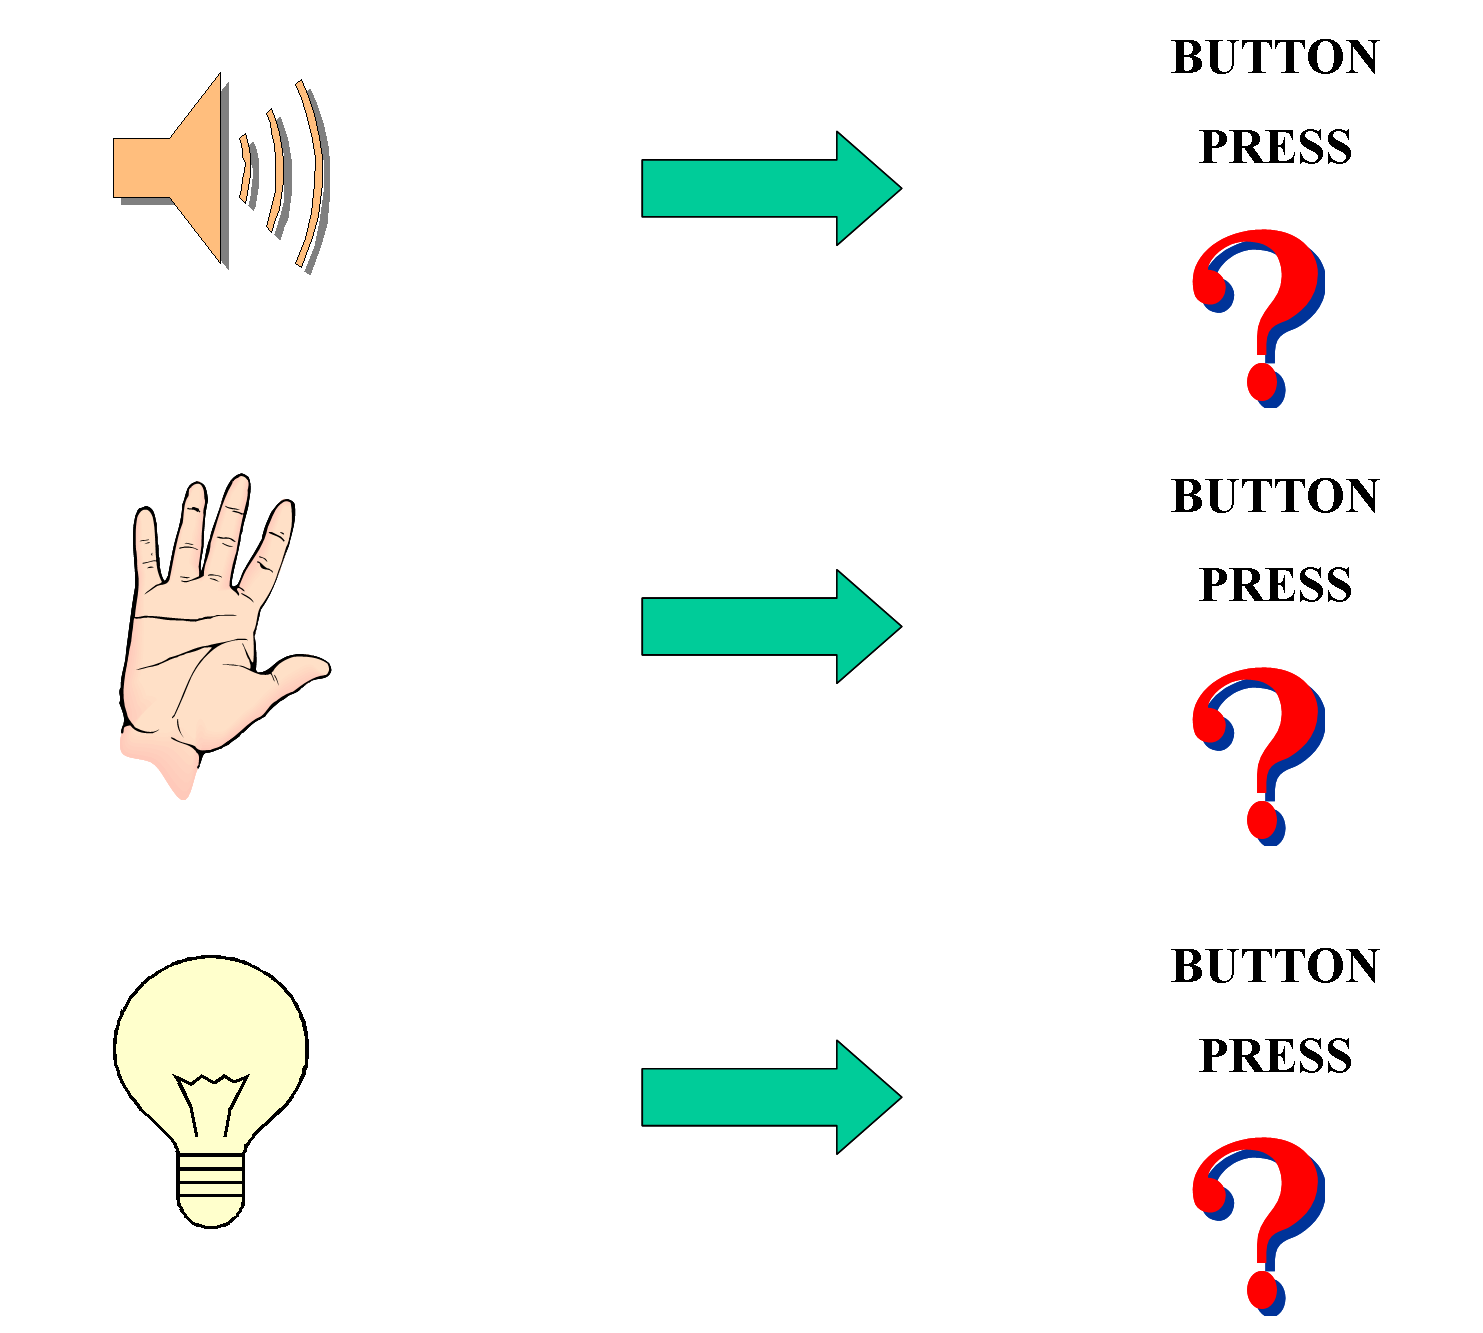
\includegraphics[width=85mm]{figures/components.eps}
%\end{center}
%\caption{Cartoon of task used to assess stimulus overselectivity (Lovaas et al, 1971).  Top panel shows a compound stimulus comprised of an auditory, tactile, and visual stimulus being associated with an action that leads to reward.  The bottom panel represents each component being tested separately in order to assess whether, individually, they have gained sufficient control over behavior to elicit a response.}
%\label{OS-Task}
%\end{figure} 


In the following we propose that deficits in PFC / DA interactions are responsible for many of the interesting behavioral patterns observed in ASD, including executive dysfunction, stimulus overselectivity, and aspects of weak central coherence.  The reduced efficacy of the DA-based gating mechanism on control representations stored within the prefrontal cortex results in overly perseverative attention.  This has two results.  First, the inability to properly adapt the control representations of the PFC produces inflexible behavior.  This behavioral perseveration is manifested in inflexible actions and is exemplified by the executive dysfunction profile in autism.  The second consequence of perturbed DA / PFC interactions is more subtle. We suggest that flexible adjustment of PFC plays an important role in shaping associational areas of cortex in a manner which affords generalization of behavior.  The lack of flexible updating of the PFC results in cortical representations that associate an overly restricted subset of environmental features with appropriate behaviors (e.g. overselectivity).  With only the restricted subset of cues dominating behavior, generalization will be hindered in situations not containing the associated and restricted subset of features.  The resulting learning deficits can be seen in both tests of stimulus overselectivity and in measures of prototype extraction during category learning.  Failure to appropriately update the contents of PFC can also result in an inability to appropriately use temporally extended context information, explaining observed deficits in sequential implicit learning tasks and in the use of sentential context to disambiguate words. 

Next we provide important background information about autism spectrum disorders, a a more detailed description of the interactions between mid-brain dopamine system and the PFC, as well as a brief survey of previous computational modeling efforts seeking to explain behavior of people with autism.  After the relevant background is covered, we summarize using computational modeling techniques how dysfunctional interactions between the DA system and the PFC can account for a wide range of behaviors in people with ASD including Executive Dysfuncion, overselectivity, implicit learning deficits, difficulty with lexical disambiguation, as well as prototype formation.  

